\section{Principes généraux du \textit{deep learning} liés au TAL}

Les statistiques ont intéressé relativement tôt plusieurs branches des sciences humaines, dont celles du domaine classique avec l'histoire quantitative ou la linguistique de corpus. Les statistiques ont alors un rôle relativement simple: permettre d'observer des phénomènes à distance du texte ou des données récoltées par l'histoire, et établir ainsi des règles par exemple. On peut citer comme exemple UN TRAVAIL UTILISANT LA STATISTIQUE SUR L'ORDRE SVO EN FRANCAIS (?). Depuis maintenant plusieurs décennies, on s'est aussi rendu compte dans ces mêmes domaines que les mathématiques et l'informatique offraient d'autres possibilités, en particulier ce que l'on appelle l'\textit{apprentissage machine} (\textit{machine learning}): il devient possible d'enseigner à un programme à analyser des phénomènes, par exemple syntaxiques ou sémantiques. Pour faire cela, les programmes se composent d'ensemble de formules mathématiques comprenant des variables qui, en voyant des données, vont s'adapter à ces dernières pour reconnaître comme l'être humain des motifs permettant de les classer. Si l'on apprenait à la machine à reconnaître des noms propres, le premier indice serait souvent une majuscule à l'initiale: c'est un premier motif validant l'hypothèse.

L'apprentissage machine commence par l'entraînement: il faut donner à la machine des données, lui dire quelle est la réponse attendue. C'est le même phénomène avec les enfants en bas âge et l'acquisition du langage: à force de répéter que tel objet est une voiture, l'enfant intègre "Machine à 4 Roues" = Voiture. La machine va pendant cet entraînement modifier les variables qui constituent son modèle mathématique: en somme, c'est toujours la même formule qui est appliquée, mais la machine va décider au fur et à mesure de l'importance de chacune des informations. Par exemple, pour les noms propres, elle comprendra peu à peu que l'information position dans la phrase et majuscule à l'initiale sont très importantes, tandis que les suffixes ne le sont pas forcément... Ces valeurs de variables de l'algorithme sont appelées \textit{poids} ou \textit{paramètres} et constituent une retranscription mathématique de ce que la machine a appris. 

\begin{figure}[h]
    \centering
    \begin{equation*}
        \begin{matrix}
            \textrm{\textit{Mot}} \\
            \begin{bmatrix}
            \textrm{Commence par une majuscule} \\
            \textrm{Premier mot dans la phrase} \\
            \textrm{Précédé d'une préposition} \\
            \textrm{...} \\
            \end{bmatrix}
        \end{matrix}
        \rightarrow
        \begin{matrix}
            \textrm{Fortissimi sunt Belgae} \\
            \begin{bmatrix}
            1 & 0 & 1 \\
            1 & 0 & 0 \\
            0 & 0 & 0 \\
            & \textrm{...} & \\
            \end{bmatrix}
        \end{matrix}
        \rightarrow Algorithme \rightarrow
        \begin{matrix}
            \textrm{Résultat} \\
            \begin{bmatrix}
            0 & 0 & 1 \\
            \end{bmatrix}
        \end{matrix}
        \end{equation*}
    \caption{Exemple de représentation de la phrase "Fortissimi sunt Belgae.". Les trois colonnes représentent les données, les lignes représentent des variables (on parle aussi de \textit{features}). Le résultat est une matrice à une seule dimension (un vecteur) comprenant 1 pour les noms propres, et 0 pour les autres.}
    \label{fig:deep-learning:matrice}
\end{figure}

Pour représenter les données, et pour effectuer des calculs dessus, l'apprentissage machine se base sur l'algèbre linéaire: il s'agit d'une partie des mathématiques considérant les nombres sous la forme de matrices et de vecteurs. Les matrices correspondent plus ou moins à des tableaux de données: elles sont réparties sur plusieurs dimensions, la plus facile à représenter pour nous étant les matrices à deux dimensions (\textit{cf.} Table \ref{fig:deep-learning:matrice}). En effet, un tableau, avec x colonnes et y lignes est tout simplement une matrice à 2 dimensions (x, y). Les colonnes et les lignes forment alors des associations qui mathématiquement permettent de mettre en exergue des informations supplémentaires.

En traitement automatique des langues, on a recourt à l'apprentissage machine pour deux grands types de tâches:
\begin{itemize}
    \item \textbf{La classification} de valeurs. Il peut s'agir de chercher à annoter des mots comme noms propres, comme adjectifs, comme sujet, etc. ou encore de classer des phrases par thèmes ou des textes par auteurs.
    \item \textbf{La génération} de texte. Elle est désormais commune dans la traduction automatique, mais aussi dans la création de robot de discussion pour les plateformes en ligne. On distinguera les générations caractère par caractère des générations mot par mot, chacune possédant des facultés différentes: la possibilité pour l'une de trouver de nouvelles formes morphologiques, pour l'autre, l'impossibilité de proposer un mot inexistant.
\end{itemize}{}

En pleine croissance depuis une dizaine d'années, l'apprentissage profond se distingue dans l'apprentissage machine principalement sur deux points: d'une part, l'absence de nécessité pour le développement d'un modèle de faire le tri manuellement parmi les données à prendre en compte (on parle d'absence de \textit{feature extraction}); d'autre part, parce que la machine ingère plus de données, elle a besoin d'une architecture mathématique plus complexe et donc de beaucoup plus de puissance de calcul. Certaines tâches, comme l'attribution d'auteur, existent à la fois comme tâche classique et comme tâche d'apprentissage profond. En apprentissage machine "classique", on sélectionne entre autres les mots les plus fréquents de la langue, les mots outils (déterminants, verbes d'état, conjonctions de coordination, etc.) et on récupère leur fréquence dans chaque texte à classer\footnote{Il existe bien d'autres paramètres utilisables, \textit{cf.} \cite{Cafieroeaax5489}}. Dans le domaine latin, en poésie latine pour être précis, les formations rythmiques\footcite{nagy_metre_nodate} ont pu être utilisées comme variables d'entrée et produire des résultats très pertinents. Au contraire, en apprentissage profond, on aura tendance à fournir le texte de manière brute ou un minimum prétraité (selon que l'on s'intéresse aux caractères plutôt qu'aux mots). C'est par exemple le procédé proposé par Ruder et al. \footcite{ruder_character-level_2016} dans une étude sur l'attribution d'auteurs sur Twitter: pour gérer des textes courts, avec des orthographes variées, leur proposition fut de prendre le texte brut et de traiter les caractères en brut comme données d'entraînement. Il reste au programme de faire le travail, par conjectures, d'identification des motifs importants.

On distingue parmi ces catégories de l'apprentissage machine deux approches exclusives: les méthodes non supervisée et supervisée. Tout comme l'humain, ces programmes sont capables de rapprocher des éléments ensemble: si un objet possède quatre roues, des portes, il est probable qu'il s'agisse de la même chose, les camions et les voitures possèdent donc une proximité, il n'est pas nécessaire de dire qu'il s'agit de véhicules. Mais elle peut aussi apprendre par injonction et correction: une automobile et un carrosse ont 4 roues, mais on enseigne à la machine qu'ils représentent deux catégories distinctes d'objet. La différence fondamentale entre les deux protocoles réside dans la présence dans les données fournies à l'entraînement des résultats attendus. Fondée sur leur absence, la méthode non supervisée va effectuer des rapprochements entre les données par assimilation: en traduction automatique, du français vers l'anglais par exemple, la machine repèrera facilement que la présence de \textit{est} se traduira par une présence de \textit{is}. En traitement automatique du langage et en apprentissage profond, cette méthode est principalement utilisée, outre le cas précédent, pour créer des corpus: on le retrouve par exemple sur des agrégateurs tels que \textit{Google News} où les articles sont rassemblés par thème en fonction de la proximité de leur sujet. Il n'y a pas - ou peu - d'éditorialisation humaine dans ce genre de procédé. Au contraire, en supervisé, on donnera à la machine à reconnaître Molière de Corneille en lui disant: ce texte est de Corneille, ce texte est de Molière, etc. 

Pour être précis, pour cette dernière méthode, la machine joue en quelque sorte à un jeu de chaud et froid avec les données: à chaque fois qu'elle donne une réponse, elle est comparée à la réponse attendue. L'écart entre ces réponses est une mesure mathématique appelée \textit{loss} (perte). Cette perte est d'ailleurs transmise à l'algorithme pour affiner ses poids, et le programme a alors pour objectif de réduire cet écart le plus possible: on appelle cela la \textit{rétropropagation} (\textit{backpropagation}). Un entraînement va voir ces données plusieurs fois, jusqu'à atteindre une impossibilité d'apprendre plus: on appelle ces cycles de consultation des \textit{epochs} (époques). Comme avec un enfant en bas âge, la répétition permet à la machine d'assimiler les motifs et de proposer les réponses attendues en s'y adaptant mathématiquement. Une fois le modèle entraîné, il peut être utilisé sur des données sans réponse connue: on parle alors d'inférence ou de prédiction, et le modèle n'apprend plus.

\begin{table}[h]
\centering
\begin{tabular}{lllccc}
\toprule
\multirow{2}{*}{Texte} & \multirow{2}{*}{Étiquette réelle}& \multirow{2}{*}{Étiquette de prédiction} & \multicolumn{3}{l}{Catégorie de classification} \\
                       &                         &                             & Corneille        & Molière       & Racine       \\ \midrule
Le Cid                 & Corneille               & Corneille                   & VP               & VN            & VN           \\
Le Misanthrope         & Molière                 & Molière                     & VN               & VP            & VN           \\
Phèdre                 & Racine                  & Racine                      & VN               & VN            & VP           \\
L'Avare                & Molière                 & Racine                      & VN               & FN            & FP          \\ \bottomrule
\end{tabular}
\caption{Exemple de classification avec les catégories afférentes. VP = Vrai Positif, FP = Faux Positif, VN = Vrai Négatif, FN = Faux Négatif}
\label{deep-learning:table:true-positives}
\end{table}

Pour mesurer l'efficacité d'un modèle supervisé, on le teste. Pour cela, on coupe généralement un corpus de données entre des données d'entraînement (\textit{train data}) et de test (\textit{test data}). On compare ensuite chacune des prédictions du modèle obtenu avec les étiquettes données dans le corpus, que l'on appelle vérité de terrain (\textit{ground truth}). Les étiquettes sont regroupées en classes: par exemple, dans le cas de Molière et Corneille, nous avons deux classes, et si nous avons 128 textes, nous avons 128 étiquettes réparties entre ces deux classes. Les résultats sont regroupés ensuite dans 4 catégories (\textit{cf.} \ref{deep-learning:table:true-positives}): les vrais positifs (VP/TP, bonne étiquette), faux positifs (FP, mauvaise étiquette pour la classe actuelle), vrais négatifs (VN/TN, reconnu comme n'étant pas de cette étiquette), faux négatif (FN, étiquette de la classe actuelle non reconnue); si toutes les étiquettes sont dans les catégories qualifiées de vraies, le modèle n'a fait aucune erreur. Ces écarts à la vérité sont mesurés principalement par 4 formules qui fournissent des pourcentages (100\% étant le meilleur score):
\begin{itemize}
    \item L'\textit{accuracy}\footnote{Le choix a été fait de ne jamais traduire \textit{accuracy} en raison de sa traduction en "précision" qui crée la confusion avec l'autre mesure \textit{precision}} mesure le nombre de vrais positifs sur le nombre total d'éléments annotés, et on pourrait le ramener à un pourcentage classique de bonne réponse. En machine learning, on le définit aussi par la formule correspondante $accuracy = \frac{VP + VN}{VP + VN + FP + FN}$
    \item La \textit{precision} mesure le pourcentage de bonnes réponses par classe sur l'ensemble des attributions effectuées sur cette classe. Elle favorise les attributions correctes à une classe sans prendre en compte les non-attributions. Sa formule est $precision = \frac{VP}{VP + FP}$
    \item Le \textit{recall} (rappel) mesure le pourcentage de réponses correctes sur l'ensemble de la classe. Elle favorise la reconnaissance de chacune des classes plutôt que les mauvaises attributions. Sa formule est $recall = \frac{VP}{VP+FN}$.
    \item Le F-Score (qui peut se découper en F1-, F2-, etc.) est la moyenne harmonique de la précision et du rappel, offrant ainsi une mesure intermédiaire. Sa formule est $F1 = \frac{2 \cdot precision\cdot recall}{precision+ recall}$
\end{itemize}{}

\label{deep-learning:overfitting}
Un risque de l'entraînement est de se retrouver avec un modèle qui apprend les réponses par coeur pour chaque donnée d'entrée: à ce moment-là, il sera incapable de gérer des données extérieures. Une des sources du problème peut être un corpus d'entraînement trop homogène: la catégorie nom propre ne comprend que des phrases où les noms propres sont précédés d'une abréviation (M., Mme, etc.), la machine apprend qu'un nom propre nécessite leur présence. On appelle cela un phénomène de \textit{surspécialisation} (\textit{overfitting}) au corpus d'entraînement\footnote{Par ailleurs, le phénomène étant clairement dû au corpus dans cet exemple, on parle aussi de biais de corpus.}. Sans que cela soit toujours le cas, une \textit{accuracy} à 100\% sur un corpus d'entraînement ou une loss de 0 est souvent l'un de ces signes. Pour éviter cela, on peut faire appel à plusieurs stratégies, non exclusives:
\begin{itemize}
    \item l'utilisation d'un corpus de développement ou d'évaluation (\textit{dev/eval corpus}). Il est vu lors de l'entraînement, mais n'est pas utilisé pour l'apprentissage: les erreurs ne sont pas individuellement transmises à l'algorithme. Cependant, sa perte, ou toute mesure sélectionnée dans ce cadre sont utilisées comme grand indicateur de fonctionnement: si le corpus d'entraînement fait 100\%, mais que le corpus de développement fait 80\%, on indiquera au modèle qu'il faut continuer à apprendre, quitte à s'éloigner des 100\%.
    \item l'utilisation, dans l'architecture du modèle, de \textit{dropout}, c'est-à-dire la suppression aléatoire d'une partie des données d'entraînement à chaque époque. En traitement automatique de la langue, il s'agit principalement de supprimer un mot par exemple.
\end{itemize}


\begin{figure}[h]
    \centering
    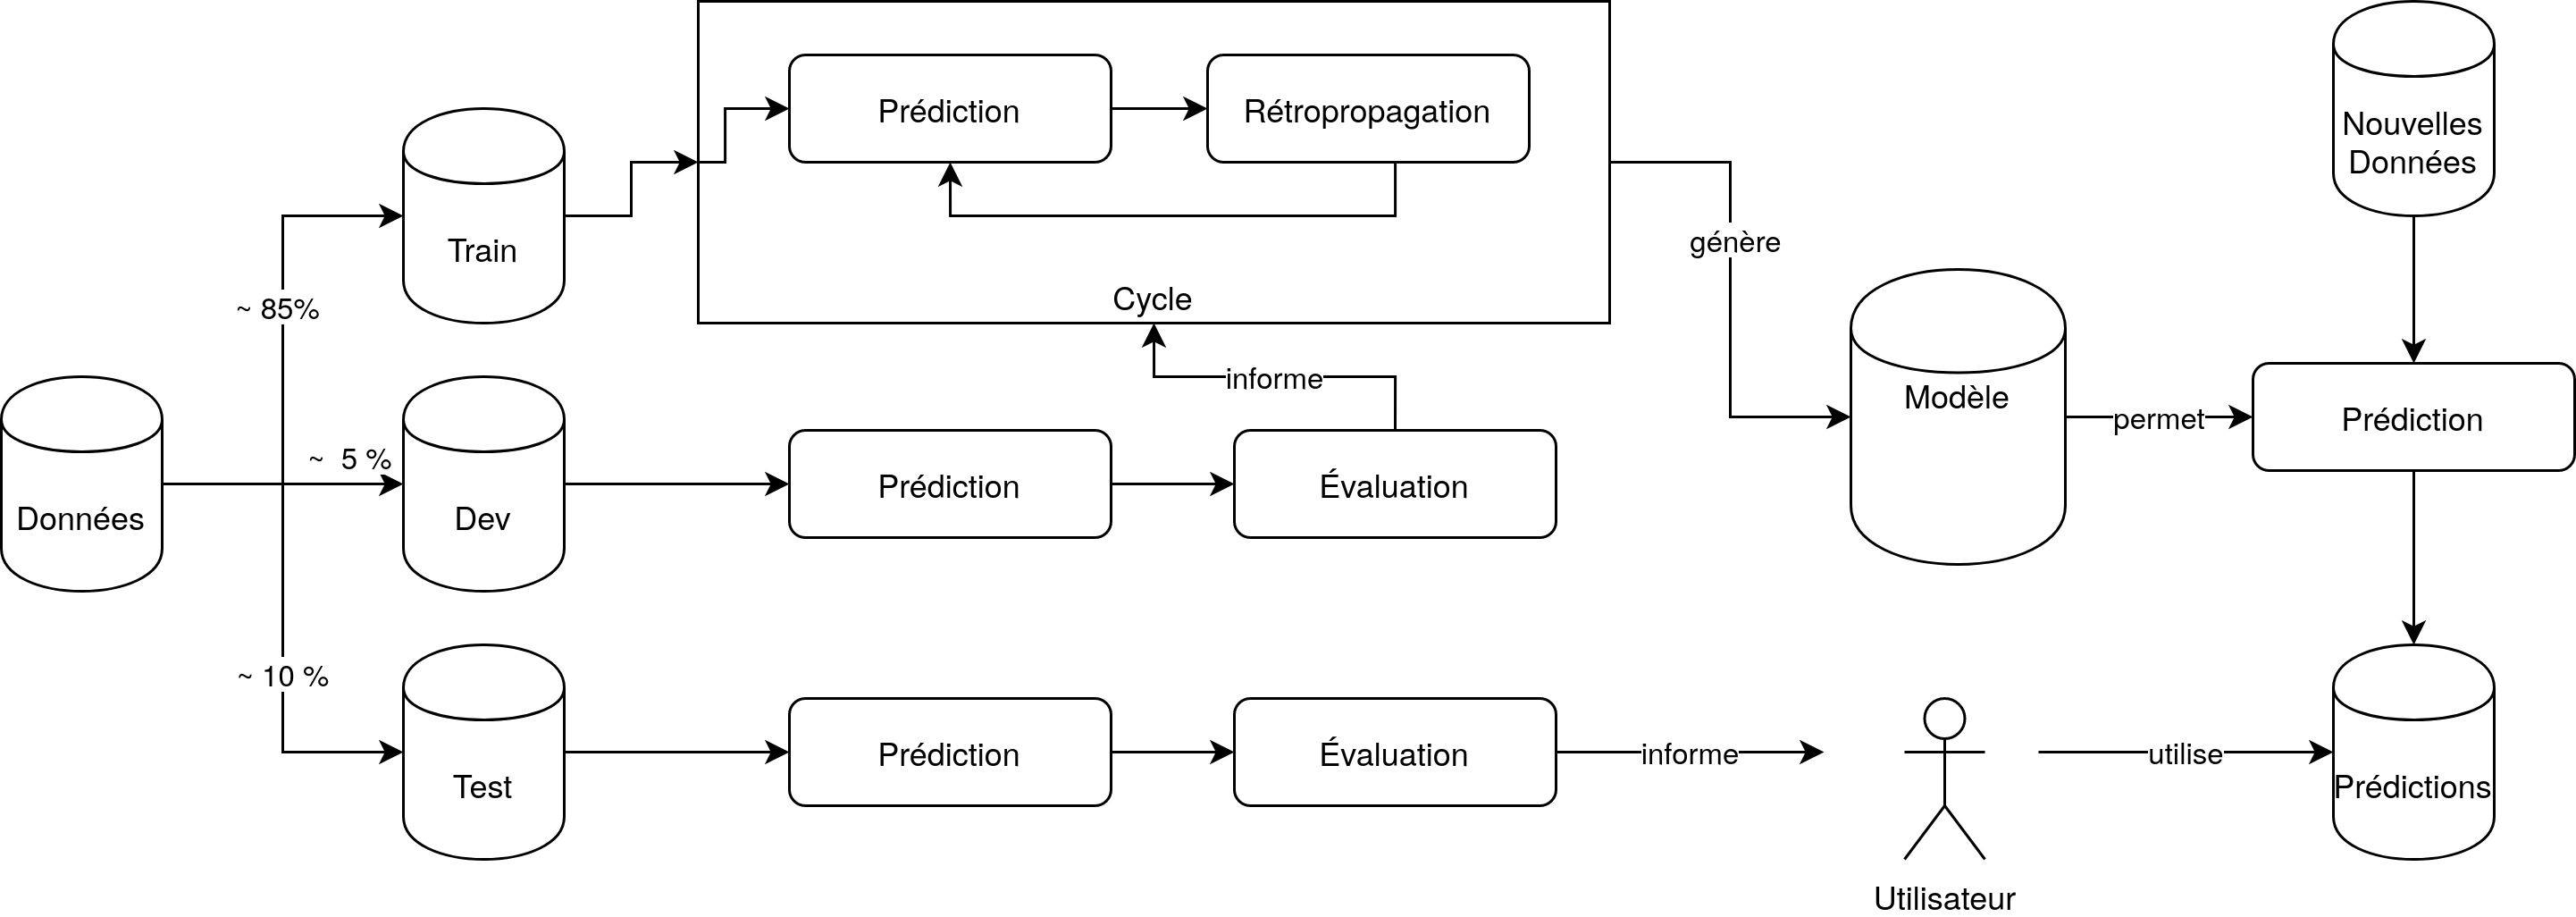
\includegraphics[width=\linewidth]{results/deep-learning/explanations/MachineLearning.png}
    \caption{Étapes, rôles et fonctionnement de l'apprentissage machine supervisé.}
    \label{fig:deep-learning:fonctionnement}
\end{figure}

Enfin, on parle ici et là d'hyperparamètres d'architecture: il s'agit principalement de variables de configuration qui, pour un modèle, changent l'architecture ou sa manière de s'entraîner. L'un d'eux, très commun, est nommé \textit{learning rate}: il s'agit d'un nombre (principalement un décimal, de type 0.001) qui sert de pas pour corriger les erreurs du modèle. Plus il est bas, plus le modèle met de temps à apprendre; plus il est haut, plus le modèle risque de rater la bonne direction d'apprentissage. D'autres hyperparamètres concernent généralement la taille des réseaux neuronaux qui composent l'architecture. 

On retrouve en traitement automatique des langues quelques modules d'architecture très communs que l'on se propose d'expliquer, en partie, ici. Ces modules sont très souvent combinés ensemble: il est rare de voir une architecture complètement basée sur un seul de ces éléments.

\subsection{Embeddings}
\label{deep-learning:embeddings}

Une première difficulté pour la machine est de comprendre ce qu'est un mot. Puisque la machine, pour son calcul, doit opérer par nombres, la première option est donc de dire: à chaque mot, un chiffre. Si l'on a deux phrases, par exemple "\textit{fortissimi sunt belgae}" et "\textit{timendi sunt belgae}", à chaque mot nouveau un chiffre serait attribué, et l'on donnerait à l'algorithme les nombres 1, 2 et 3 puis 4, 2, 3: 2 et 3 sont présents deux fois, on ne réattribue pas d'identifiant numérique à \textit{sunt} et \textit{belgae}, par contre, \textit{timendi} qui est nouveau poussera à la création d'un nouvel identifiant, 4. On appelle ces nombres valeurs symboliques, et le résultat final \textit{one-hot vector}. Enfin, l'index des mots est considéré comme une variable discrète: son nombre de possibilités est fini (on peut les énumérer)\footnote{Une variable discrète est une variable dont on peut énumérer les valeurs (1, 2, 3, 4, etc.). par opposition à une variable continue (0.000000001, 0.000000002, etc.)}. Malheureusement pour la machine, ce caractère discret de la variable rend très difficile de faire un rapprochement entre 4 (timendi) et 1 (fortissimi): ils n'ont mathématiquement rien à voir ensemble. 

Dans notre langage, nous utilisons en fait déjà une forme de mathématisation des sens. Les expressions du type "\textit{timendi} est proche de \textit{fortissimi}" sont des métaphores de spatialisation: si l'on devait dessiner une carte des mots des deux phrases de l'encodage précédent, notre approche serait sûrement de rapprocher les deux précédents tandis que \textit{sunt} et \textit{Belgae} seraient autre part sur la carte. Faire cela, c'est projeter sur deux dimensions d'un plan (x et y) les sens des mots. On peut pousser cela en 3 dimensions, 4 dimensions, etc. Si chacune de ces colonnes était une catégorie de sens, on pourrait alors affiner et représenter chacun de ces mots (\textit{cf.} Figure \ref{figure:deep-learning:projection-embedding}). Bien sûr, ces colonnes ne sont pas aussi simplement lisibles, mais font suffisamment sens pour que la machine en fasse usage: cette représentation que la machine construit est issue d'un module de réseau que l'on appelle \textit{embeddings}\footnote{Par habitude, on appelle aussi le produit du réseau \textit{embeddings}.}. 

Au fur et à mesure de l'apprentissage, la machine fige alors une représentation de chacun des mots qui sera utile au reste du réseau (\textit{cf.} figure \ref{figure:deep-learning:embeddings-encoding}). Dans l'exemple précédent, on établit une matrice de $N$ par $M$, où $N$ correspond au nombre de mots différents rencontrés (ici 4) et $M$ une dimension de projection choisie (ici 2). La matrice d'embeddings, si l'on avait par exemple un apprentissage en vue d'une classification par sens ou d'une classification par nature de mot, aura tendance à proposer des résultats tels que dans la figure précédente, avec un rapprochement évident pour l'être humain, mais aussi désormais pour la machine de \textit{timendi} et \textit{fortissimi}. La machine apprend alors à reconnaître des éléments par leur contexte: pour des mots, ce principe repose sur le principe de distributionnalité\footcite{firth_papers_1957} qui veut que deux mots se ressemblant (sémantiquement, syntaxiquement, etc.) aient le même contexte\footnote{Nous proposons une étude de ce qu'apprend l'algorithme en fonction de la tâche en \ref{subsec:lemma_resultats}.}.

% Exemple d'encodage one hot

\begin{figure}
    \centering
    \noindent\begin{minipage}{.32\linewidth}
        \begin{equation*}
            \begin{bmatrix}
            fortissimi \\ 
            sunt \\ 
            Belgae \\ 
            timendi \\ 
            ... \\ 
            ... \\ 
            ... \\ 
            \end{bmatrix}
            \rightarrow \begin{bmatrix}
            1 \\ 
            2 \\ 
            3 \\ 
            4 \\ 
            ... \\ 
            ... \\ 
            n \\ 
            \end{bmatrix}
        \end{equation*}
    \end{minipage}%
    \begin{minipage}{.32\linewidth}
        \begin{equation*}
            \begin{matrix}
            \textrm{Fortissimi sunt Belgae}\\ 
            \textrm{Timendi sunt Belgae}
            \end{matrix}
            \rightarrow
            \begin{matrix}
            \left [ 1\;  2\;  3 \right ]\\ 
            \left [ 4\;  2\;  3 \right ]
            \end{matrix}
        \end{equation*}
    \end{minipage}
    \caption{Exemple d'encodage\textit{ one-hot}. On constitue d'abord un dictionnaire de transcodage, puis on traduit à l'aide de celui-ci les phrases}
    \label{deep-learning:one-hot-encoding}
\end{figure}

\begin{figure}[h]
    \centering
    \noindent\begin{minipage}{.45\linewidth}
        \resizebox{\linewidth}{!}{%
            \begin{tabular}{l|lll}
             & Féminin & Jeunesse & Royal \\ \midrule
            Homme                          & 0       & 0        & 0     \\
            Femme                          & 1       & 0        & 0     \\
            Garçon                         & 0       & 1        & 0     \\
            Fille                          & 1       & 1        & 0     \\
            Prince                         & 0       & 1        & 1     \\
            Princesse                      & 1       & 1        & 1     \\
            Reine                          & 1       & 0        & 1     \\
            Roi                            & 0       & 0        & 1     \\
            Monarque                       & 0.5     & 0.5      & 1    
            \end{tabular}%
        }
    \end{minipage}
    \begin{minipage}{.45\linewidth}
        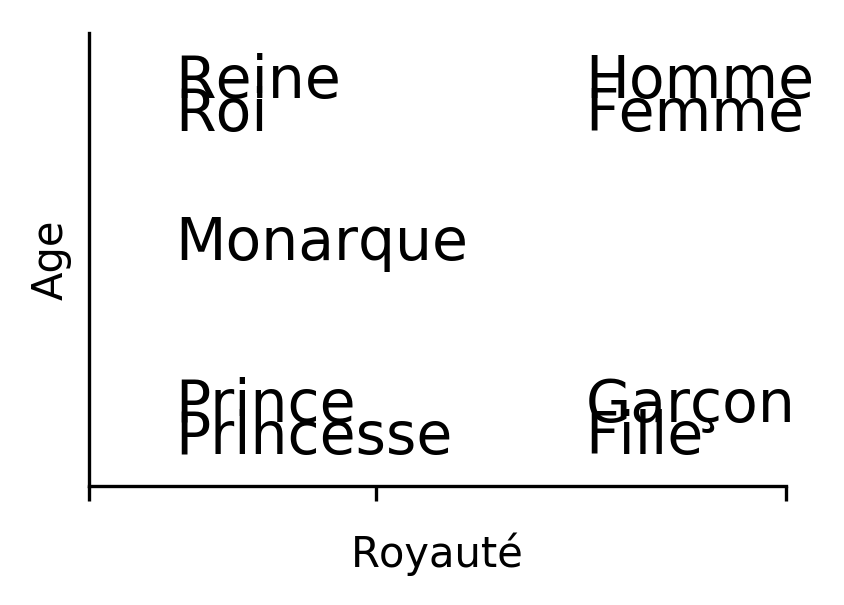
\includegraphics[width=\linewidth]{figures/chap2/visualisation_embedding.png}
    \end{minipage}
    \caption{En choisissant des catégories adaptées, il est possible de placer dans un tableau tout un ensemble d'informations et de différencier des éléments de vocabulaire mathématiquement. Ici, \textit{monarque} est neutre, il n'est donc ni féminin (1) ni masculin (0). Une fois ces catégories choisies, on peut les représenter sur deux dimensions via PCA. On remarque alors que les groupes se rassemblent. Inspiration: Lynn, Shane\footcite{lynn_get_2018}}
    \label{figure:deep-learning:projection-embedding}
\end{figure}

\begin{figure}[h]
    \centering
    \noindent\begin{minipage}{.32\linewidth}
        \begin{equation*}
            \begin{matrix}
            Fortissimi \\ 
            sunt \\ 
            Belgae \\ 
            timendi \\ 
            ... \\ 
            ... \\ 
            ... \\ 
            \end{matrix}
            \rightarrow 
            \begin{bmatrix}
            0.97 & 0.85 \\ 
            0.12 & 0.85 \\ 
            0.54 & 0.28 \\ 
            0.92 & 0.90 \\ 
            ... & ... \\ 
            ... & ... \\ 
            n & ... \\ 
            \end{bmatrix}
        \end{equation*}
    \end{minipage}%
    \begin{minipage}{.32\linewidth}
        \begin{equation*}
            \begin{matrix}
                \textrm{Fortissimi sunt} \\ 
                \textrm{Belgae} \\ \\
                \textrm{Timendi sunt} \\
                \textrm{Belgae}
            \end{matrix}
            \rightarrow
            \begin{matrix}
            
            \begin{bmatrix}
            0.97 & 0.85 \\ 
            0.12 & 0.85 \\ 
            0.54 & 0.28 \\ 
            \end{bmatrix} \\ \\
            
            \begin{bmatrix}
            0.92 & 0.90 \\
            0.12 & 0.85 \\ 
            0.54 & 0.28 \\ 
            \end{bmatrix}
            
            \end{matrix}
        \end{equation*}
    \end{minipage}
    \caption{Remplacement de l'encodage one-hot par une couche  embedding. La proximité entre les vecteurs de \textit{Fortissimi} et \textit{Timendi} et la répétition des deux autres mots produisent deux phrases très proches mathématiquement.}
    \label{figure:deep-learning:embeddings-encoding}
\end{figure}

Bien sûr, les dimensions des embeddings sont ordinairement beaucoup plus grandes que dans l'exemple construit ici: David Bamman, lors de la création d'une telle matrice sur l'ensemble des mots présents dans les livres classés langue latine du site archives.org\footcite{bamman_11k_2012}, a créé une matrice de $N=2,961,867$ et de $M=100$ (100 est une dimension assez habituelle pour $M$). 

\subsection{Réseaux Linéaires}
\label{deep-learning:linear}

Si les \textit{embeddings} permettent de générer une représentation des données, les modèles \textit{linéaires}\footnote{On le retrouve sous plusieurs noms: \textit{perceptron}, \textit{linear network}, \textit{dense layer}, \textit{régression linéaire}, etc.} permettent de les classer. Ce modèle est l'élément le plus simple d'un réseau neuronal (\textit{cf.} figure \ref{fig:deep-learning:simple-linear}). Par ailleurs, une couche linéaire peut être accumulée à d'autres couches linéaires, souvent en réduisant peu à peu la taille du réseau jusqu'à arriver à la taille de sortie: cela s'appelle un \textit{perceptron multicouche}. Par exemple, pour un classement de texte par auteur, on pourrait créer un réseau utilisant les fréquences de chacun des mots présents comme donnée d'entrée (fréquence de "fortissimi", "belgae", etc. dans chacun des textes) et qui viendrait réduire, sur plusieurs couches, la taille de la matrice jusqu'à obtenir la taille des réponses possibles (\textit{eg.} Nombre de mots -> 512 dimensions -> 256 dimensions -> 128 dimensions -> 2 si deux auteurs).Le perceptron multicouche (\textit{multi layer perceptron}) constitue le réseau neuronal le plus simple possible (\textit{cf.} figure \ref{fig:deep-learning:mlp}). Dans une telle situation, les couches intermédiaires sont appelées \textit{hidden layers}. Son principe de réduction des dimensions peut aussi être appliqué à des sorties d'autres modules avant une classification finale.

\begin{figure}[h]
    \centering
    \noindent\begin{minipage}{.35\linewidth}
        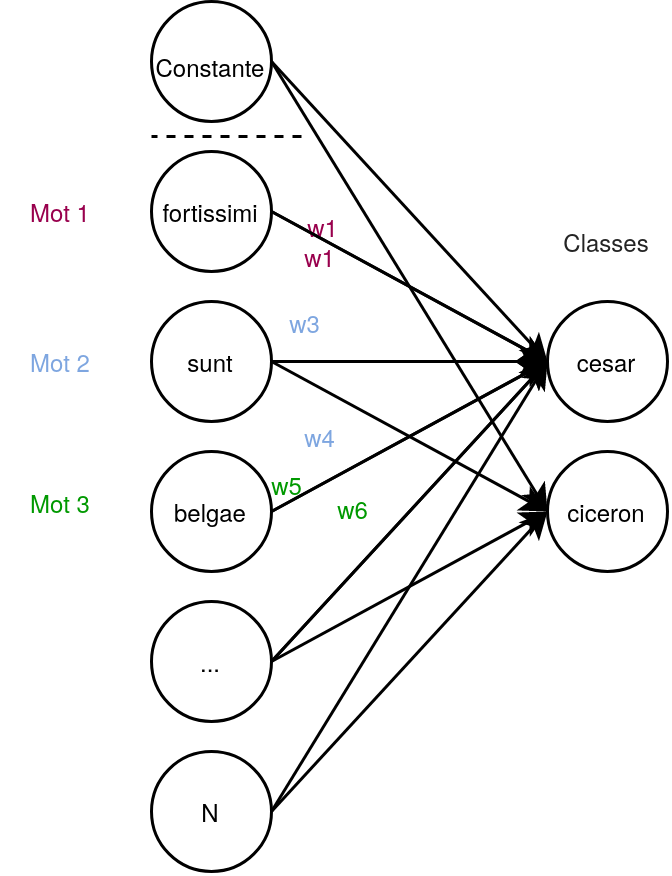
\includegraphics[width=\linewidth]{results/deep-learning/explanations/SimpleLinear.png}
        \caption{Exemple de couche linéaire (simplifiée)}
        \label{fig:deep-learning:simple-linear}
    \end{minipage}%
    \hspace{0.04\linewidth}
    \noindent\begin{minipage}{.60\linewidth}
        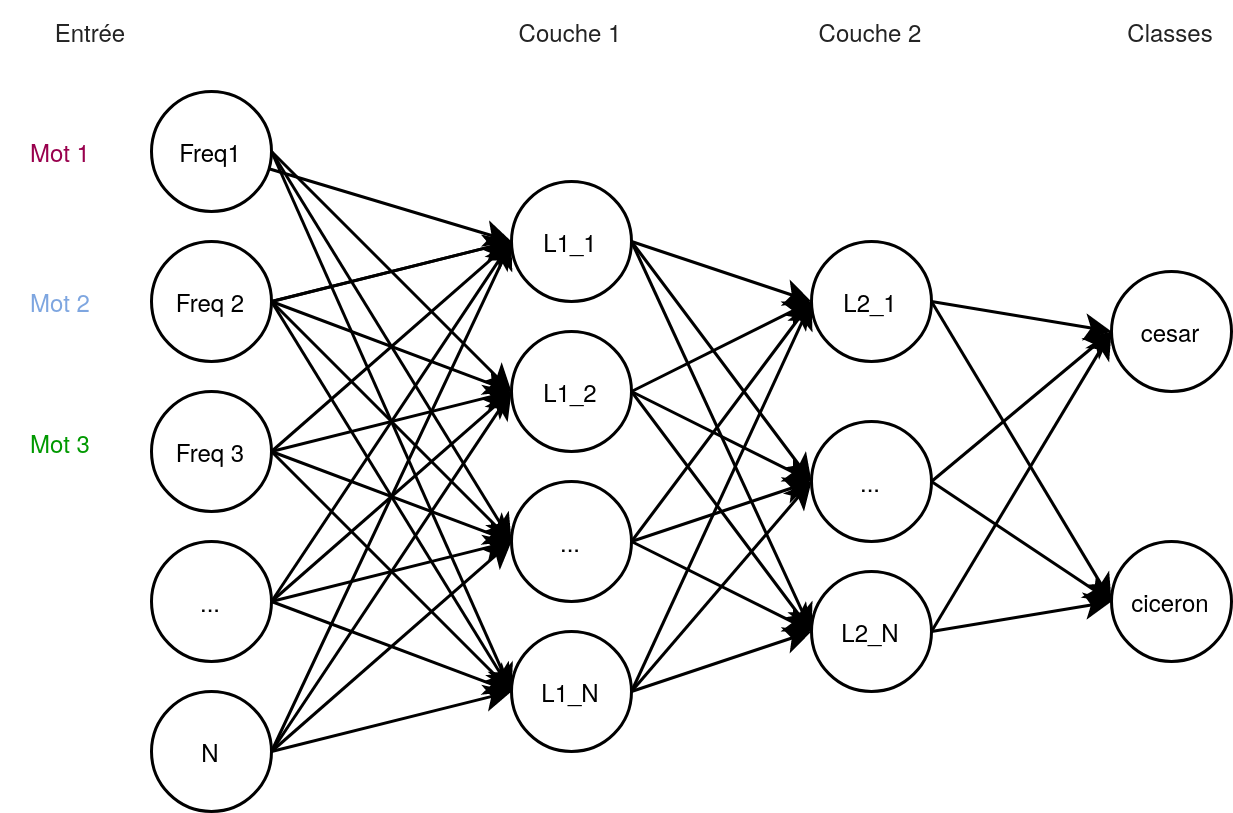
\includegraphics[width=\linewidth]{results/deep-learning/explanations/MLP.png}
        \caption{Exemple de perceptron multicouche. Le réseau construit ici possède une entrée de taille N, une sortie de 2, et un réseau $Linear(N, L1_N) \rightarrow Linear(L1_N, L2_N) \rightarrow Linear(L2_N, 2)$}
        \label{fig:deep-learning:mlp}
    \end{minipage}%
\end{figure}

Les couches linéaires prennent une forme mathématique très simple. Dans le cadre d'un vecteur de fréquence comme dans la figure \ref{fig:deep-learning:mlp}, le perceptron prend une matrice de taille $M$ par 1 (le vecteur) et ressort une matrice de taille $M...O$ où $O$ est le nombre d'auteurs. Sur ce vecteur, le modèle n'applique qu'une fonction affine. À chaque valeur $M_{i}$ (ici, $i$ est un index de mot), et pour chaque classe de sortie notée $j$, on associe un poids $w_{ij}$ en plus d'une variable partagée par chaque classe appelée \textit{biais} ($b_{j}$) telle que $f(X, j) = W_{j} \dot X + b_{j}$  où X est la matrice de données fournie\footnote{En algèbre linéaire, une multiplication de matrice A, de taille N par M, par une matrice B, de taille M par P, résulte en une matrice de taille N par P: une multiplication peut donc réduire la deuxième dimension d'une matrice ou l'augmenter.}.


\subsection{Réseaux Neuronaux Acycliques (RNN; LSTM et GRU)}

Malheureusement, les couches linéaires posent un problème, en particulier pour les TALs et le traitement d'image: il ne traitent pas vraiment les données en séries. Les perceptrons multicouches ne gèrent l'ensemble des données que comme un ensemble de phénomènes plus ou moins indépendants et, dans tous les cas, non séquentiels. On appelle ce type de réseau \textit{feed-forward} (propagation directe). Pour traiter des données en séries, on s'est d'abord tourné vers d'autres types de réseaux, appelés \textit{réseaux neuronaux acycliques (recurrent neural networks, RNN)}. Les réseaux récurrents ont la particularité de traiter les données en séries, et de réutiliser l'analyse de chaque élément pour l'analyse de l'élément suivant, comme le montre le schéma en \ref{fig:deep-learning:rnn}.

\begin{figure}[h]
    \centering
    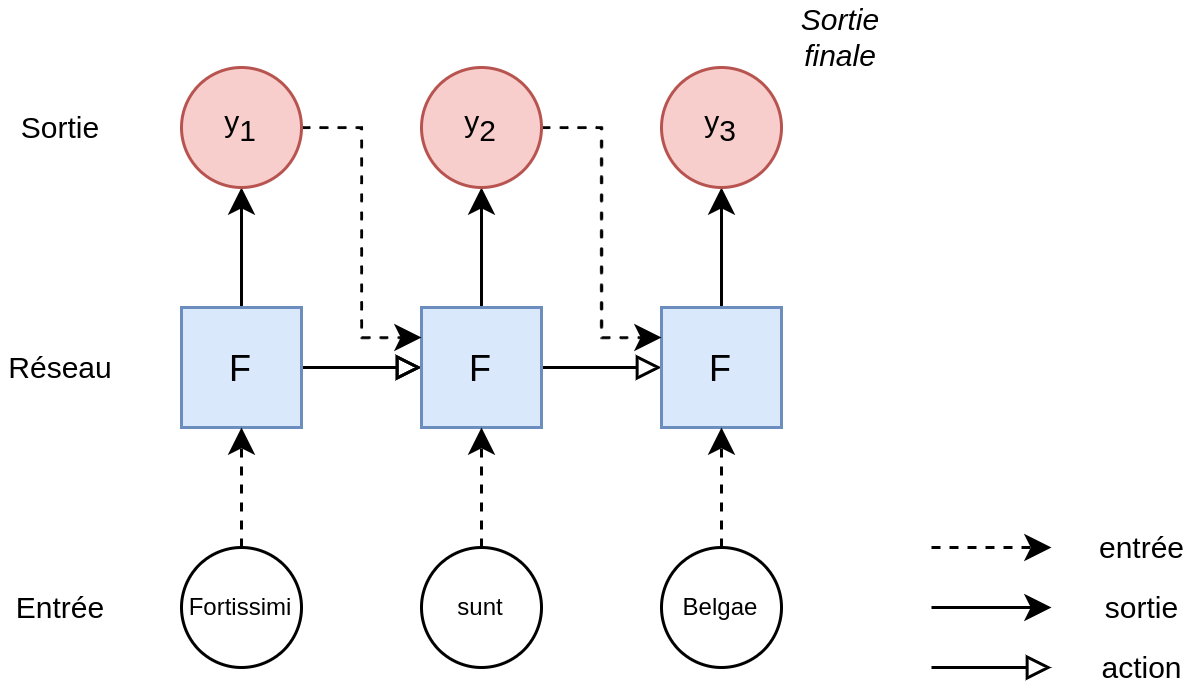
\includegraphics[height=5cm]{results/deep-learning/explanations/RNN.png}
    \caption{Exemple de réseau acyclique}
    \label{fig:deep-learning:rnn}
\end{figure}

\begin{figure}[h]
    \centering
    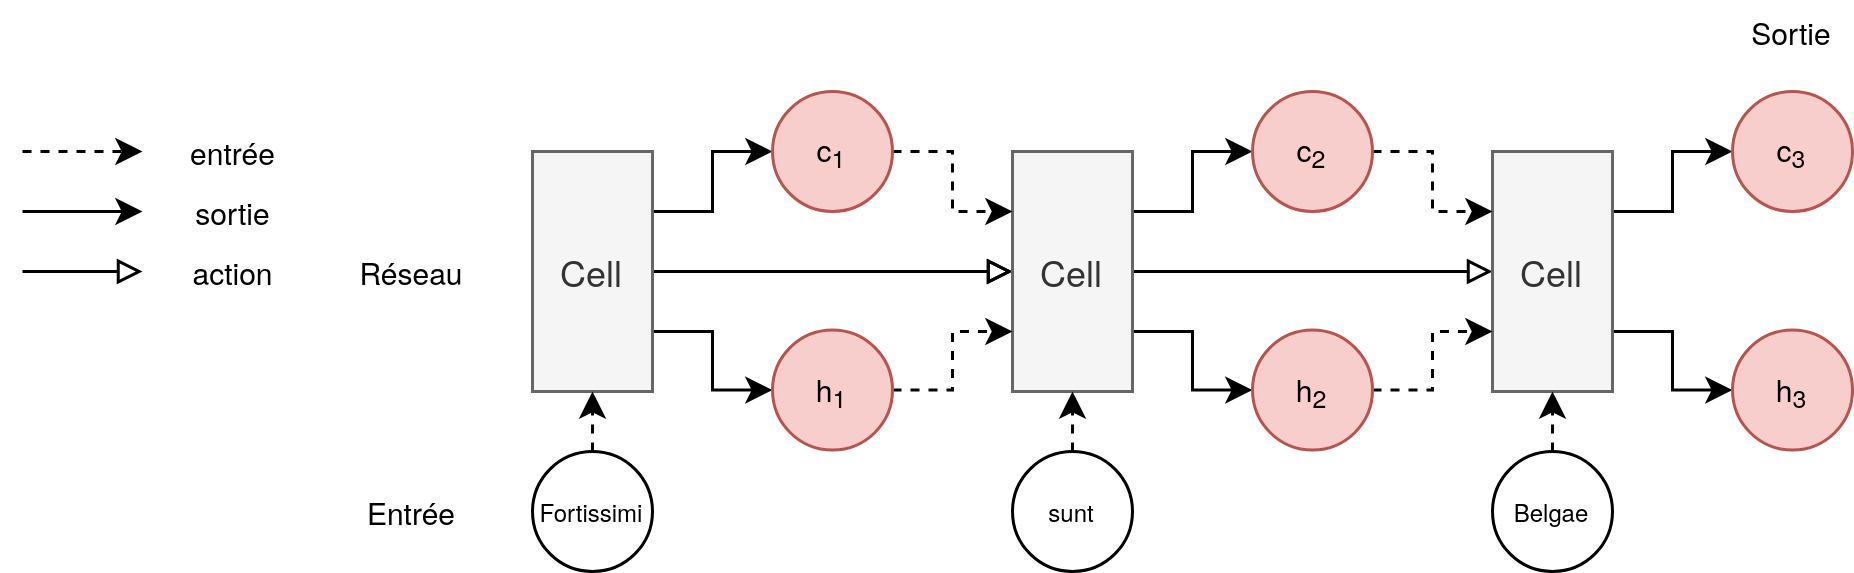
\includegraphics[width=\linewidth]{results/deep-learning/explanations/LSTM-Zoom-Out.png}
    \caption{Plusieurs cellules de LSTM}
    \label{fig:deep-learning:lstm}
\end{figure}

Le problème des réseaux acycliques classiques se trouve dans la rétropropagation: alors que l'algorithme va propager les informations sur les erreurs rencontrées, cette donnée de correction va peu à peu perdre de sa valeur. En somme, les derniers mots d'une phrase sont plus corrigés que les premiers mots de celle-ci. Pour éviter un tel problème, Sepp Hochreiter et Jürgen Schmidhuber ont proposé les réseaux Long Short-Term Memory (LSTM)\footcite{hochreiter_long_1997}. Ils partent du principe que dans une séquence, tout n'est pas nécessaire. Ainsi, dans la phrase "Caesar sum et fortissimi sunt Belgae", si je m'intéresse au narrateur, deux voire trois mots ont de l'importance: \textit{Belgae, sum, Caesar}. Il n'est donc pas nécessaire de s'intéresser à toutes les valeurs... Pour corriger cela, ils introduisent, en plus des valeurs de sorties (\textit{hidden state}, notée $y$ dans la figure \ref{fig:deep-learning:rnn}, très souvent notée $h$) une mémoire appelée \textit{cell state} (notée $C$). À partir de ces deux valeurs calculées et des valeurs d'entrées, le réseau peut alors effectuer des filtres et prendre en compte les valeurs qui précèdent ou les ignorer. Il existe trois filtres:
\begin{itemize}
    \item la \textit{forget gate}. Elle a pour but de nettoyer la mémoire engrangée dans la \textit{cell state} en fonction de la valeur d'entrée et de l'\textit{hidden state} précédent. 
    \item l'\textit{input gate}. Elle a pour rôle de filtrer dans les valeurs d'entrées celles qui doivent avoir un impact sur la mémoire.
    \item l'\textit{output gate}. En fonction de la mémoire et de la valeur nouvellement acquise de l'\textit{hidden state}, elle décide de supprimer ou non des valeurs de ce dernier.
\end{itemize}
La combinaison de ces trois systèmes aura alors pour effet de créer un environnement propice à la propagation. Cependant, à force d'accumuler dans un sens, de gauche à droite par exemple, on s'est aperçu que le résultat final accordait plus d'importance aux derniers mots qu'aux premiers. Pour corriger cela, on a proposé de faire des LSTM bidirectionnels: pour simplifier, au lieu d'avoir un seul LSTM, deux sont présents et vont dans des sens différents, puis, le résultat final est une simple concaténation des résultats individuels de ces deux LSTMs.

Dans un réseau en LSTM, on a traditionnellement accès à l'ensemble des hidden state, qui correspondent à l'encodage des mots. Si, au contraire, on s'intéresse à l'encodage de la phrase, on utilisera en général le dernier état accessible.

\begin{figure}[h]
    \centering
    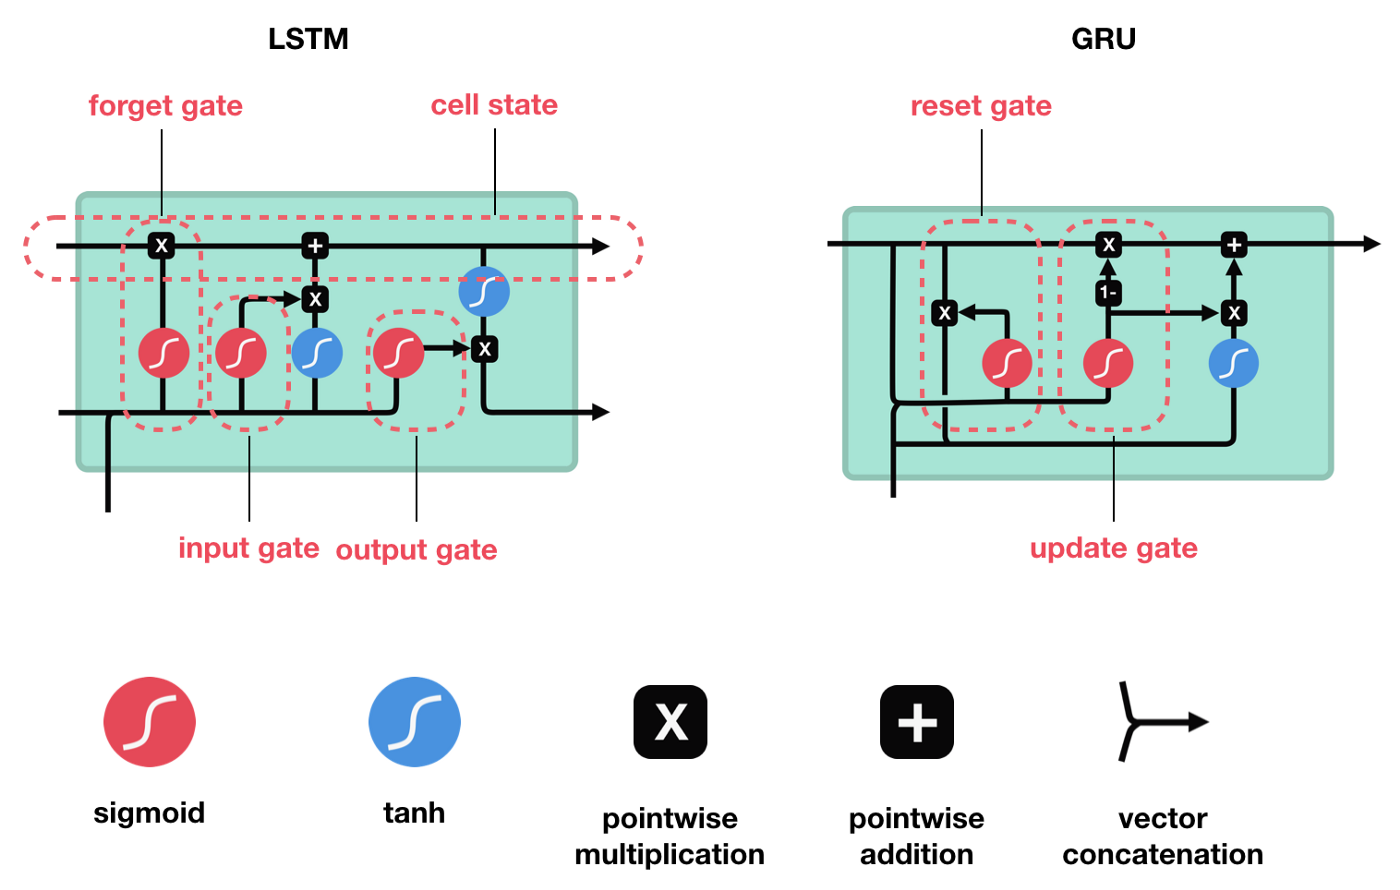
\includegraphics[height=5cm]{results/deep-learning/explanations/GRU LSTM.png}
    \caption{Fonctionnement interne d'une cellule GRU et d'une cellule LSTM. Source: \cite{nguyen_illustrated_2019}}
    \label{fig:deep-learning:lstm-gru}
\end{figure}


\label{deep-learning:gru}
Inventé en 2014 par Cho et al.\footcite{cho_properties_2014}, les \textit{Gated Recurrent Unit} (GRU) cherchent à traiter le même problème que les LSTMs. Leur différence consiste principalement dans leur nombre de filtres (2) et dans l'absence de \textit{cell state}, ce qui les rend potentiellement plus rapides. Les deux valeurs de \textit{gate}, \textit{reset} ($R_{t}$) et \textit{update} ($Z_{t}$), sont calculées en fonction de l'\textit{hidden state} précédent $H_{t-1}$ et du X courant $X_{t}$. La \textit{reset gate} est appliquée à l'hidden state précédent avant sa prise en compte pour l'\textit{hidden state} suivant, tandis que l'\textit{update gate} permet de filtrer ce qui va être ajouté du calcul sur $X_{t}$ au résultat final ($H_{t}$) et ce qui en échange doit être conservé de l'état précédent $H_{t-1}$.


\subsection{Réseaux neuronaux convolutionnels (CNN)}
\label{deep-learning:CNN}

Les réseaux neuronaux convolutionnels (\textit{Convolutionnal Neural Network}, CNN) sont des réseaux \textit{feed-forward} qui règlent le problème des perceptrons multicouches. Développés principalement pour le traitement d'images, il approche une image spatialement en analysant chaque pixel avec ce qui l'entoure pour en faire une sorte de résumé. Son résultat peut ensuite passer dans diverses couches de simplification (\textit{ReLU}) ou de réduction (\textit{Pooling}). En traitement automatique des langues, les CNN se distinguent des RNN en ce qu'ils traitent les mots en contexte indépendamment les uns des autres, tandis que les LSTM unidirectionnel par exemple accumulent les informations des mots précédents avec le mot cible, sans prendre en compte les mots à venir.

\begin{figure}[h]
    \centering
    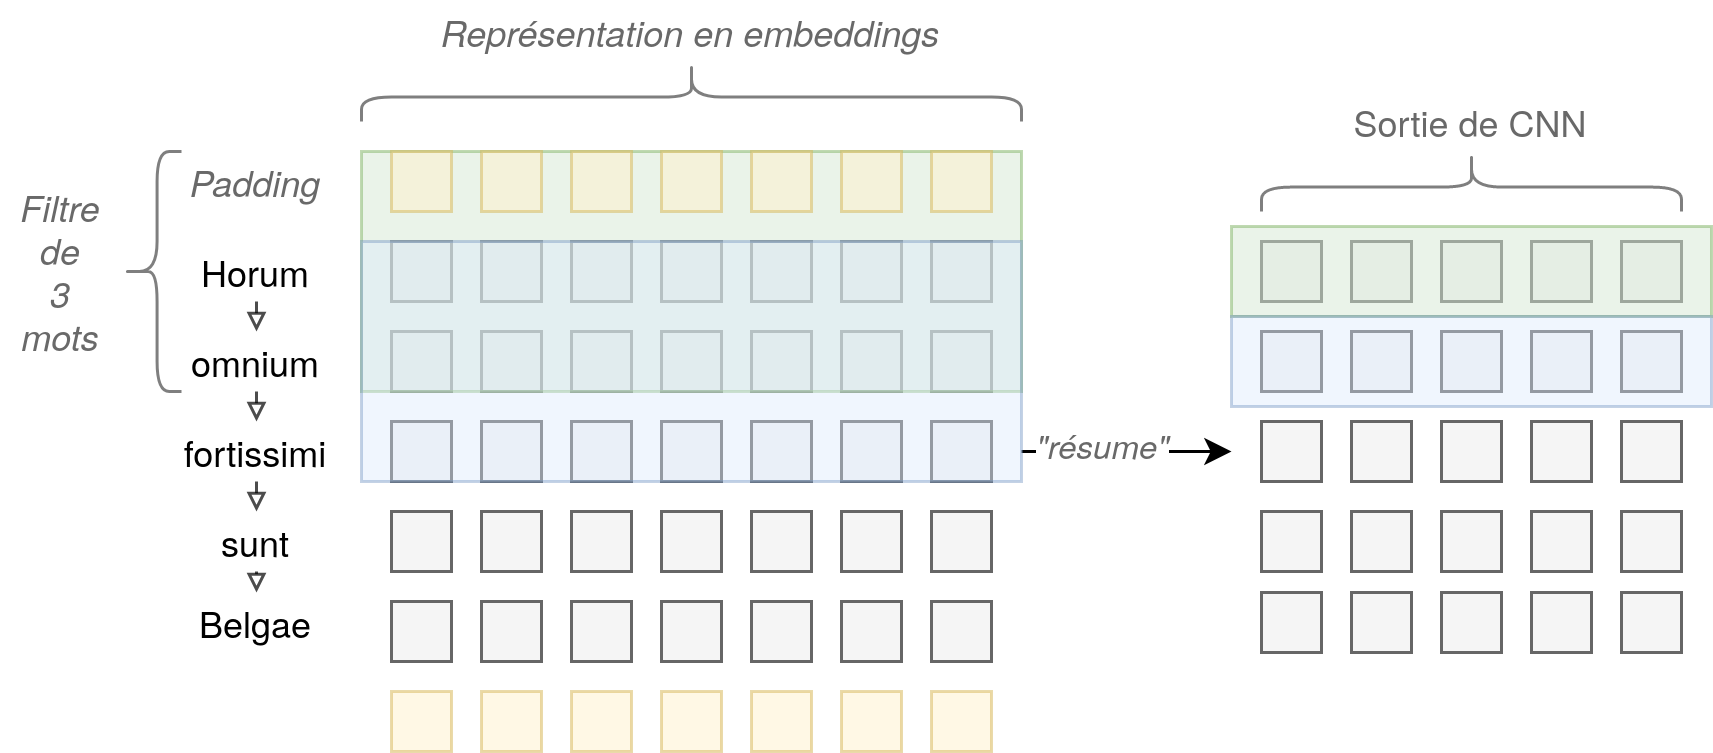
\includegraphics[width=\linewidth]{results/deep-learning/explanations/CNN.png}
    \caption{Fonctionnement simplifié et visualisation des paramètres d'un CNN.}
    \label{fig:deep-learning:cnn-tal}
\end{figure}

Un CNN est défini par sa taille de sortie, sa \textit{fenêtre}\footnote{Aussi appelé \textit{kernel, noyaux, filtre, filter}, etc.}, une \textit{marge} (\textit{padding}) et un \textit{pas} (\textit{stride}). La marge permet de prendre en compte les mots aux extrêmités de la séquence en proposant des valeurs nulles de remplissage, comme en figure \ref{fig:deep-learning:cnn-tal} (marge de 1). Le pas indique de combien de mots la fenêtre avance: par défaut, elle avance de 1. 

\subsection{Architectures Encodeur-Décodeurs}
\label{deep-learning:encoder-decoder}

Les architectures encodeur-décodeur (\textit{encoder-decoder} sont des architectures très récentes et qui ont connu en traitement automatique du langage un succès particulier. Les articles qui les ont popularisés, comme \textit{Attention Is All You Need}\footcite{vaswani_attention_2017} ou celui du modèle Bert\footcite{devlin_bert_2019}, datent en général des dernières années. Leur principe repose principalement sur une architecture dans laquelle un ensemble de RNN (en général) va produire une représentation des données en entrée qui est ensuite réutilisée par un second ensemble de RNN dont la tâche est de produire des données en sortie. Cette architecture est majoritairement utilisée dans la génération de texte, que cela soit en traduction automatique ou en légendage d'image. Nous proposons une lecture linguistique du produit en figure \ref{fig:deep-learning:encoder-decoder} où nous comparons le résultat de sortie d'un encodeur à une forme de signifié: désincarné, l'état produit par l'encodeur ne correspond plus à langue d'entrée et à ses signifiants, mais ne correspond pas non plus encore aux signifiants de la langue de sortie.

\begin{figure}[h]
    \centering
    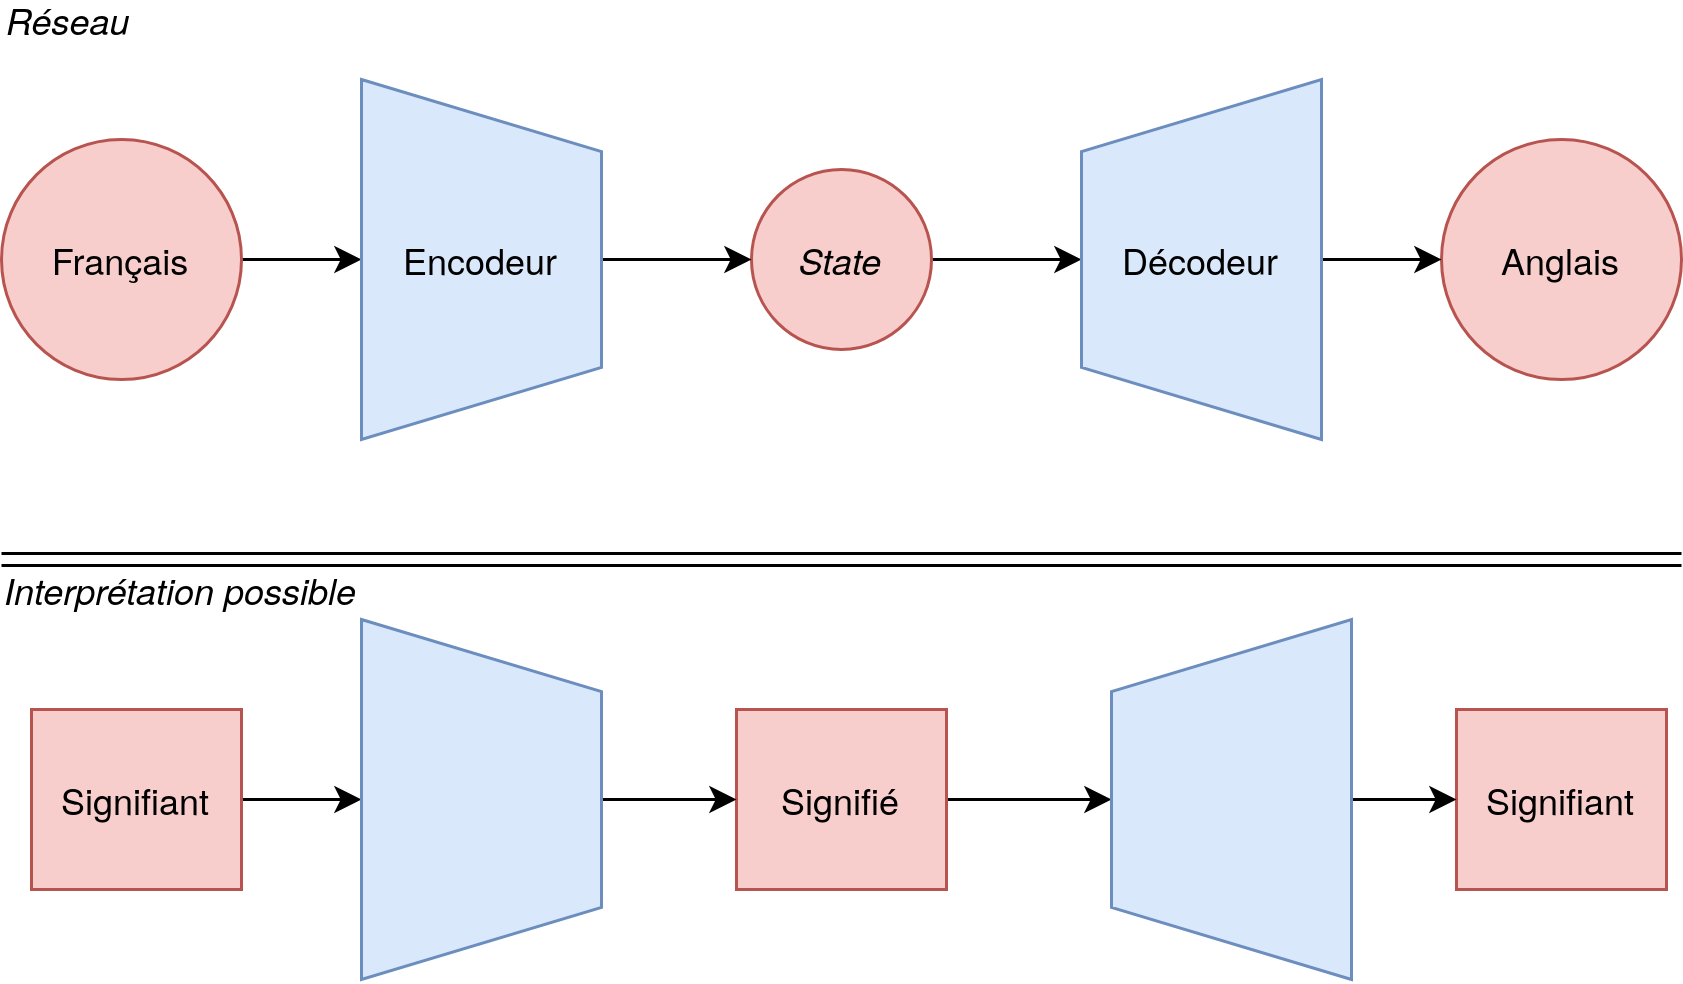
\includegraphics[width=\linewidth]{results/deep-learning/explanations/EncodeurDecodeur.png}
    \caption{Proposition d'interprétation d'une architecture encodeur-décodeur dans le cas d'une traduction automatique entre anglais et français.}
    \label{fig:deep-learning:encoder-decoder}
\end{figure}
